\documentclass[conference,a4paper]{IEEEtran}
\usepackage{cite}
\usepackage{amsmath,amssymb,amsfonts}
\usepackage{graphicx}
\usepackage{textcomp}
\usepackage{xcolor}
\usepackage[hidelinks]{hyperref}

\begin{document}

\title{Visual Dock-Velocity Feedforward for ROV Docking to a Moving Station: Failure Mechanism, Feedforward Redesign and Estimator Robustness}

\author{\IEEEauthorblockN{1\textsuperscript{st} Chak Wang Choi}
\IEEEauthorblockA{\textit{School of Mechanical and Manufacturing Engineering} \\
\textit{UNSW Sydney}\\
Sydney, Australia \\
z5413670@ad.unsw.edu.au}
\and
\IEEEauthorblockN{2\textsuperscript{nd} William J.B. Midgley}
\IEEEauthorblockA{\textit{School of Mechanical and Manufacturing Engineering} \\
\textit{UNSW Sydney}\\
Sydney, Australia \\
w.midgley@unsw.edu.au\\
ORCID: 0000-0003-3786-1691}
}

\maketitle

\begin{abstract}
Moored and suspended docking stations inherit wave motion, so the terminal visual stage of underwater docking must track a moving target, and feeding the estimated dock velocity forward should help. We report simulated docking of a BlueROV2 onto a station swaying with 0.1~m amplitude at periods from 20 to 6~s, with a passive-marker vision pipeline and the production autopilot in the loop. A reactive baseline succeeds down to 8~s; a constant-velocity estimator with feedforward degrades at 10~s and fails at 8 and 6~s. Decomposing the recorded trials shows the estimator is not the cause: the dock measurement is within 1~cm of truth and the velocity state matches the true dock velocity whenever markers are visible. The feedforward instead over-drives the vehicle, because the effort-like command channel has two to four times the gain and lag it was tuned against; the vehicle over-swings the dock by up to 1.7 times, which at 6~s starves the alignment tolerance and at 8~s loses the markers, after which the filter dead-reckons on a frozen velocity state. We propose a feedforward closed on the vehicle's own velocity with a decaying velocity state during marker loss, evaluate it against the baseline, the original method and an oracle feedforward, and show by replay under correlated navigation error that a relative-frame estimator removes the velocity jitter but not the bias, which only the closed loop cancels.
\end{abstract}

\begin{IEEEkeywords}
underwater docking, remotely operated vehicle, visual servoing, moving target, Kalman filter, velocity feedforward, plant identification
\end{IEEEkeywords}

\section{Introduction}

Docking lets a resident underwater vehicle recharge and offload data without surfacing; the riskiest part is the final metres, flown on the forward camera. Real stations move: a suspended tether management system followed its vessel's heave by 1.1~m at 8.5~s \cite{trslic2020vision}, and a moored station follows the wave orbital motion at its depth, of order 0.1~m at shelf depth for the 5 to 20~s periods that carry wave energy \cite{holthuijsen2007waves}; the mean sea off New South Wales is 1.6~m at 8~s \cite{short1992wave}.

Docking control literature treats the dock as a fixed pose. Trslic et al.\ servoed reactively on the latest pose \cite{trslic2020vision} and later predicted cage heave, but from a dock-side pressure sensor and offline \cite{trslic2020neuro}. No prior work, to our knowledge, estimates a dock's wave-frequency motion onboard through vision and closes a feedforward loop on it. This paper does so for the passive-marker terminal stage of a low-cost ROV, reports that the obvious design fails at short periods, and traces the failure to its actual cause.

\section{System and Feedforward Architecture}

The vehicle is a BlueROV2 Heavy in Gazebo with the production ArduSub firmware software-in-the-loop \cite{blue2024software}. Nine size-graded ArUco markers \cite{garrido2014automatic} are fused by inverse-variance weighting after spatial-consensus outlier rejection into a nine-state error-state Kalman filter over dock position, dock velocity and a small-angle attitude correction \cite{sola2017quaternion}, run either \emph{static}, with zero velocity process noise (a constant-position filter), or \emph{sway}, with white-acceleration noise that estimates dock velocity \cite{barshalom2001estimation}. A state machine sequences coarse approach, align-then-advance and seat, with position-based visual servoing on the body-frame pose error \cite{chaumette2006visual}. In the sway regime the filter velocity is rotated into the body frame, clamped, ramped in with distance and added to the command. The command channel is effort-like: the autopilot maps it to thrust, so vehicle velocity follows with a gain and lag that must be identified, not assumed.

\section{Docking Envelope and Failure Evidence}

The sweep covers periods $\{20,16,12,10,8,6\}$~s at 0.1~m orbital amplitude, three start phases per cell, replicated on a second host (Fig.~\ref{fig:pdock}); a trial succeeds if the vehicle enters the 0.15~m aperture without first contacting the structure. The baseline docks in every trial down to 8~s; at 6~s two of three brush the aperture at 0.03 to 0.06~m/s. The feedforward method matches it to 12~s, degrades at 10~s and fails at 8 and 6~s, the band of the mean New South Wales wave period. Retuning the process noise and bounding the velocity state did not move the cliff.

\begin{figure}[t]
\centerline{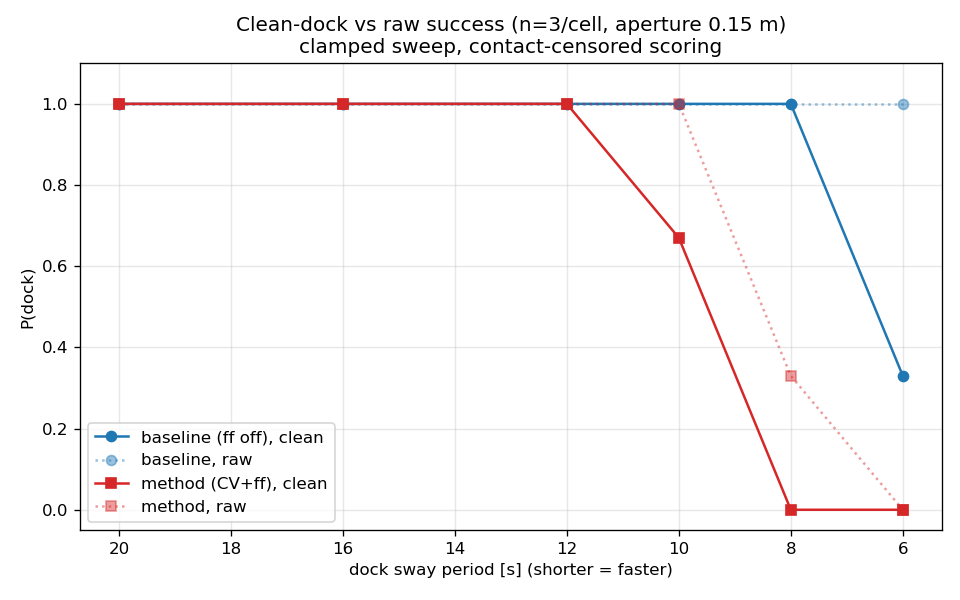
\includegraphics[width=0.52\columnwidth]{figures/clean_pdock.png}}
\caption{Docking success versus sway period, reactive baseline versus constant-velocity filter with feedforward; raw (dotted) and contact-censored (solid) scoring.}
\label{fig:pdock}
\end{figure}

We first suspected ego-motion leaking into the world-frame measurement through the vehicle's own pose. Rebuilding the measurement the filter ingested from the recorded transforms rejects this: its error against the true dock is 0.2 to 0.9~cm RMS in all 36 trials, uncorrelated with vehicle position, velocity, range or marker count. While markers are visible the filter tracks the dock to within 1~cm and its velocity state matches the true dock velocity (amplitude ratio 0.99 to 1.17, correlation 0.88 to 0.97) at every period.

What separates the regimes is the vehicle's response (Fig.~\ref{fig:mech}). With feedforward the lateral command is dominated by the feedforward term, and the vehicle's amplitude over the dock's grows from 1.06 at 20~s to 1.7 at 8 and 6~s, whereas the baseline stays between 0.9 and 1.05. Open-loop step tests identify the command channel as a first-order lag with gain 2.7~m/s per unit command and a 0.4~s time constant, against the 1.3 to 1.6 and 0.24~s the feedforward was calibrated to, so the feedforward alone drives the vehicle at 1.6 times the dock velocity in the coarse phase and 2.7 times it at the unit gain of the fine phase, where the failures occur, pulled back by the position feedback only to the measured 1.7; retuning the estimator's process noise changes neither the velocity state nor the over-swing. At 6~s the over-swing alone keeps the relative error above the 3~cm alignment tolerance, so the vehicle never advances. At 8~s the over-swing at 0.2~m range carries the markers out of view; the filter reports stale, the controller holds, and the filter integrates its frozen 0.023~m/s velocity state for 49~s to a metre off, the ``phantom dock velocity'' seen in the estimate. The excursion does not drive the vehicle, since the controller ignores a stale estimate, but it misleads every velocity-based diagnostic.

\begin{figure}[t]
\centerline{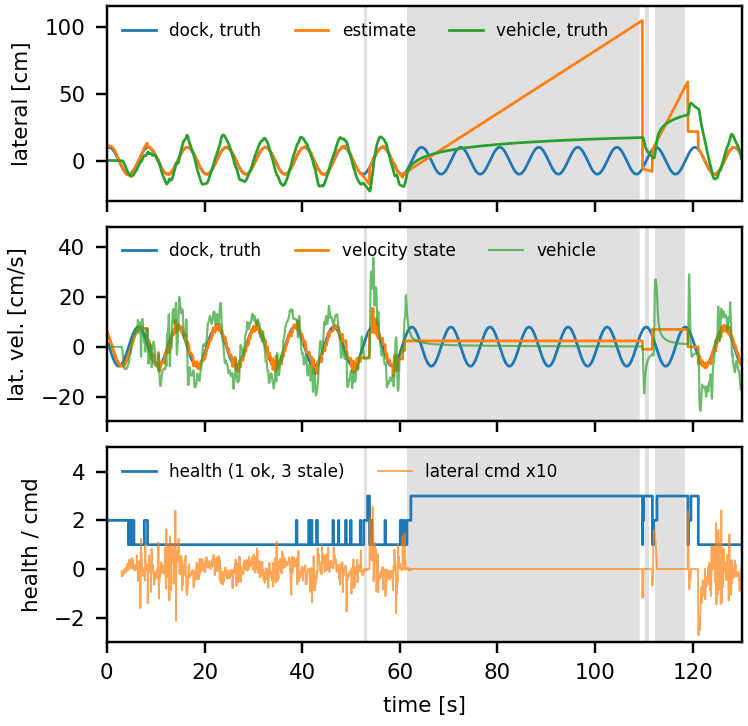
\includegraphics[width=0.74\columnwidth]{figures/mechanism_p8.png}}
\caption{Failed feedforward trial at 8~s. Top: lateral position of the true dock, the estimate and the vehicle; the estimate sits on the dock while the vehicle over-swings, then dead-reckons when markers are lost (shaded). Middle: the velocity state tracks the true dock velocity; the vehicle's is twice it. Bottom: filter health and lateral command; the command is zero throughout the blackout.}
\label{fig:mech}
\end{figure}

\section{Proposed Redesign and Evaluation Plan}

The estimator is retained. Two changes address the mechanism: the feedforward becomes a velocity setpoint closed by a loop on the vehicle's odometry velocity, so the plant gain no longer enters; and the velocity state decays after one second without an update, which cuts the replayed blackout excursion from 112 to 33~cm. Over the same periods, three phases per cell and 82 trials on one host, the redesigned feedforward docks without contact at every phase from 20 to 8~s with entry-plane offsets under 2~cm and no over-swing (vehicle-to-dock amplitude 0.9 to 1.3), where the original fails every trial at 8 and 6~s; an oracle feedforward from ground-truth dock velocity over-swings exactly as the original does (1.0 to 1.8 with frequency) and fails at 6~s, so the limit is the open-loop law and the plant, not the estimate. A second sweep injects three levels of first-order Gauss-Markov navigation error. Replaying both estimators on the recorded trials under that error shows that each absorbs a slow velocity bias one for one, since a camera measuring relative position cannot separate it from dock velocity, and that the relative-frame estimator removes only the jitter a world-frame filter makes from position noise; the closed velocity loop is what cancels the bias.

\section{Conclusion}

Dock-velocity feedforward cannot be added to a static-dock pipeline as an afterthought, and the reason is not the one the estimator's symptoms suggest: the feedforward, the plant gain and lag, and the marker field of view form a loop that must be designed together, and dead-reckoning during blackout must be bounded. The system's own signals pointed at the estimator; only ground truth exposed the plant, so deployments need independent verification.

\bibliographystyle{IEEEtran}
\bibliography{refs}

\end{document}
